\documentclass[10pt,twocolumn,journal]{IEEEtran}
\usepackage[utf-8]{inputenc}
\usepackage{graphicx}
\usepackage{amsmath}
\usepackage{amssymb}
\usepackage{booktabs}
\usepackage{cite}
\usepackage{hyperref}
\usepackage{pgfplots}
\pgfplotsset{compat=1.17}
\usepackage{tikz}
\usetikzlibrary{shapes, arrows}
\usepackage{xcolor}

\title{Context-Aware Neural Bandits for Adversarial Quantum Network Routing: The Capacity Paradox and Threat-Responsive Allocation}

\author{Piter Garcia,~\IEEEmembership{Student Member, IEEE}
\thanks{P. Garcia is with the Department of Computer Science, Rochester Institute of Technology, Rochester, NY 14623, USA (e-mail: pzg8794@rit.edu).}
\thanks{Manuscript received December 11, 2025; revised \today.}}

\begin{document}

\maketitle

\begin{abstract}

Most quantum network routing research assumes that entanglement success rates between nodes are known or can be accurately estimated. This assumption is unrealistic: real-world quantum networks exhibit dynamically varying link fidelities due to decoherence, hardware fluctuations, and adversarial interference. We address the online learning problem of jointly optimizing entanglement path selection and qubit allocation in real time without prior link-performance knowledge.

Through systematic evaluation across 370+ experimental conditions spanning 13 algorithms, 5 scenarios (Stochastic, Markov, Adaptive, OnlineAdaptive, Baseline), 4 allocator strategies, and 2 capacity settings at mid-range horizons (4K--8K frames), we uncover five key findings: \textbf{(1)} context-aware Pursuit neural bandits (CPursuitNeuralUCB, iCPursuitNeuralUCB) outperform classical and reward-only MABs by 18--24 pp and maintain performance floors 15--20 pp higher than adversarial-first designs; \textbf{(2)} adversarial-robust methods (EXP3, EXPNeuralUCB) achieve 10--24 pp lower efficiency than contextual variants under the very attacks they target; \textbf{(3)} ARIMA-based predictive context improves stochastic stability by +2.6 pp and reduces variance by 87\%; \textbf{(4)} the \emph{capacity paradox}—doubling replay buffer from $T_b$ to $2T$ causes 22--30 pp collapse under Adaptive attacks but yields +23 pp gains under Markov, a \textbf{48 pp swing}—reveals that resource predictability, not bandwidth, is the limiting factor; \textbf{(5)} allocator selection introduces 10--15 pp performance swings across identical algorithms, establishing algorithm-allocator co-design as critical.

We derive threat-responsive deployment rules achieving 85--92\% efficiency across scenarios versus 75--80\% for fixed-capacity baselines. These findings extend beyond quantum networks to any resource-constrained multi-armed bandit system with intelligent adversaries.

\end{abstract}

\begin{IEEEkeywords}
Quantum networks, multi-armed bandits, contextual bandits, adversarial robustness, neural bandits, dynamic resource allocation, pursuit learning, capacity allocation.
\end{IEEEkeywords}

\IEEEpeerreviewmaketitle

% ========== INTRODUCTION ==========
\section{Introduction}
\label{sec:introduction}

Quantum networks enable distributed quantum computing and sensing by establishing entangled links between remote nodes. Unlike classical networks where information flows deterministically, quantum entanglement distribution is probabilistic: each attempted path succeeds with some fidelity (typically 60--90\% in near-term repeater networks) and fails silently due to decoherence. No retransmission is possible under the no-cloning theorem, making routing decisions irreversible and high-stakes.

Two fundamental challenges arise in quantum routing. First, path selection must balance exploration of uncertain link fidelities against exploitation of known-good routes, a classic multi-armed bandit (MAB) problem complicated by non-stationary fidelities and reactive adversaries. Second, qubit allocation—how many quantum resources to dedicate to each path—is typically hardcoded at provisioning time, yet our capacity paradox shows that rigid, high-capacity allocations become exploitable vulnerabilities under adaptive attacks, collapsing performance by 22--30 percentage points.

Existing work treats these as separate problems or assumes static, benign environments. In practice, quantum network operators face both stochastic failures (natural decoherence) and strategic attacks (adversaries learning routing patterns to induce failures at critical moments). Current heuristics and fixed-capacity designs are not equipped to respond.

We systematically evaluate 13 neural bandit algorithms across 370+ experimental conditions spanning 5 uncertainty regimes, 4 allocator strategies, and 2 capacity settings. This evaluation reveals three counterintuitive insights: (1) \textbf{context-aware bandits outperform adversarial-robust methods by 10--24 pp under reactive attacks}, (2) \textbf{doubling capacity causes a catastrophic 25 pp efficiency collapse under adaptive adversaries}—a 48 pp swing from Markov's +23.3 pp gain—and (3) \textbf{allocator selection introduces 10--15 pp performance swings}, establishing algorithm-allocator co-design as essential.

We address these challenges through a unified framework: (i) contextual Pursuit neural bandits that leverage topology, fidelity, and traffic features to make routing decisions robust to both stochastic and adversarial noise, and (ii) dynamic capacity allocation that adjusts resource budgets in real time based on detected threat characteristics. The result is a threat-responsive routing system that maintains 85--92\% efficiency across diverse scenarios, compared to 75--80\% for fixed-capacity baselines.

\section{Related Work}
\label{sec:related}

\subsection{Foundational Multi-Armed Bandits (2002--2018)}

Foundational work establishes the exploration--exploitation trade-off and regret guarantees that underlie all modern bandit algorithms. Canonical results include UCB1 and Thompson Sampling with logarithmic regret $\tilde{O}\!\left(\sum_i \frac{\log T}{\Delta_i}\right)$ under i.i.d.\ rewards, and EXP3 with adversarial regret $\tilde{O}(\sqrt{T K \log K})$. These results define efficiency and robustness frontiers that any hybrid or domain-specific method must respect, independently of whether the arms represent quantum paths, financial assets, or treatment arms in clinical trials.

\subsection{Contextual and Neural Bandits (2012--2024)}

Contextual bandits extend classical MABs by conditioning decisions on observable state, enabling decisions in non-stationary and structured environments. LinUCB uses linear reward models with context-dependent confidence bounds, while NeuralUCB and NeuralTS replace linear predictors with deep neural networks and maintain uncertainty via confidence or posterior sampling in representation space. These methods show that bandits are not tied to discrete arms, but to the principle: \emph{maintain uncertainty estimates over value predictions and act optimistically or probabilistically with respect to them}. This abstraction applies directly to quantum routing, where link fidelities, queue lengths, and topology features define the context for path selection.

\subsection{Adversarial and Hybrid Robustness (2002--2024)}

Adversarial bandits such as EXP3 prioritize worst-case performance, achieving $O(\sqrt{T K \log K})$ regret at the cost of conservative behavior in benign environments. Hybrid methods (e.g., pursuit learning, EXPNeuralUCB) aim for ``best of both worlds'' behavior by combining stochastic efficiency with adversarial robustness. In practice, our experiments show that purely adversarial-first designs like EXPNeuralUCB can become unstable under complex reactive attacks and capacity shifts, achieving substantially lower efficiency than pursuit-based contextual variants in realistic quantum-routing workloads.

\subsection{Predictive and Informed Bandits (2012--2025)}

Predictive bandits incorporate explicit forecasting or world models, moving from reactive adaptation to anticipatory allocation. Examples include iCMAB, which couples contextual bandits with EXAMM-evolved RNNs, and related Bayesian or time-series-based schemes. In our work, iCPursuitNeuralUCB instantiates this idea with an ARIMA-based predictive context warmup, trading 4--10× additional runtime for zero-retry stability and higher efficiency under stochastic and adversarial noise. This demonstrates that forecasting future context (e.g., decoherence patterns and traffic bursts) can stabilize performance in regimes where purely reactive algorithms fail.

\subsection{Quantum Network Routing with Bandits (2020--2025)}

Recent quantum network studies apply bandits and reinforcement learning to routing, but typically assume static or heuristically tuned capacities and focus on small topologies. Existing work benchmarks policies under stochastic failures and simple adversaries, often treating capacity as a fixed provisioning parameter rather than an adaptive signal that can itself be exploited. Our capacity-paradox analysis shows that this assumption can be dangerously misleading: fixed high capacity (2T) improves performance in benign or structured settings but causes 22--30 percentage point collapses under adaptive attacks, motivating threat-aware, dynamically scaled bandit routing instead.

\subsection{Universal MAB Framework}

Most prior work deploys bandits as domain tools (for ads, trials, or routing). We instead present MAB as a \emph{universal} abstraction for sequential decision-making under uncertainty. The core meta-problem—balancing exploration and exploitation using uncertainty-aware value predictions—transcends domains. We operationalize this universality as a modular stack: (i) a pluggable allocator layer (UCB1, Thompson, $\varepsilon$-greedy, EXP3, NeuralUCB, pursuit, informed/predictive variants), (ii) an optional world-model/forecast layer (e.g., ARIMA or EXAMM/RNN) to anticipate nonstationarity, and (iii) a domain adapter that maps context/reward signals and constraints without altering allocator logic. By systematically comparing classical, contextual, adversarial, and predictive bandits in quantum routing, we validate the universality of MAB principles under realistic, compound uncertainty.

% ========== METHODOLOGY ==========
\section{Methodology}
\label{sec:methodology}

\subsection{Experimental Design}

We evaluate 4 primary algorithms (GNeuralUCB, EXPNeuralUCB, CPursuitNeuralUCB, iCPursuitNeuralUCB) across 370+ experimental conditions spanning:

\begin{itemize}
  \item \textbf{Algorithms (13 total):} 4 neural bandits + 9 classical baselines (UCB1, Thompson Sampling, $\varepsilon$-greedy, EXP3 variants, pursuit algorithms).
  \item \textbf{Scenarios (5):} Stochastic (6.25\% natural failure rate), Markov (25\% structured attacks), Adaptive (25\% reactive learning), OnlineAdaptive (25\% real-time learning), Baseline (0\% no attacks).
  \item \textbf{Allocators (4):} Fixed (hardcoded $T_b$), DynamicUCB (responds to efficiency), Random (control), Thompson Sampling (Bayesian posterior).
  \item \textbf{Capacity Settings (2):} $T_b$ baseline (proportional to horizon), $2T$ doubled.
  \item \textbf{Horizons (3):} 4K, 6K, 8K frames; results averaged over 3--5 runs per condition.
\end{itemize}

\subsection{Performance Metrics}

Efficiency quantifies how close an algorithm's performance approaches the theoretical optimum:
\[
\text{Efficiency} = \frac{R_{\text{algorithm}}}{R_{\text{Oracle}}} \times 100
\]
where $R_{\text{algorithm}}$ is total reward obtained and $R_{\text{Oracle}}$ is the theoretical maximum with perfect knowledge.

Coefficient of Variation (CV) measures relative variability and stability:
\[
\text{CV} = \frac{\text{StdDev}}{\text{Mean}} \times 100
\]
Lower CV indicates more stable operational performance. Win Rate is the percentage of scenario-allocator combinations where an algorithm achieves best performance.

\subsection{Network Topology and Fidelity Model}

We use a 4-node diamond topology with 4 quantum paths and 35 total qubits distributed per allocator strategy. Link fidelities initialize uniformly (70--85\%) and degrade over time according to coherence models. Attack models inject failures at specified rates; Adaptive and OnlineAdaptive attackers observe allocation patterns and adjust strategy to maximize loss.

% ========== RESULTS ==========
\section{Results}
\label{sec:results}

\subsection{RQ1: Context-Aware Models Lead}

Context-aware Pursuit models (CPursuitNeuralUCB: 89.4\%, iCPursuitNeuralUCB: 87.1\%) outperform neural non-context baselines (GNeuralUCB: 83.0\%, EXPNeuralUCB: 77.6\%) by 6--12 percentage points in stochastic scenarios and exceed classical reward-only bandits by 18--24 points. This advantage stems from Pursuit algorithms' use of topology and channel-quality features for path selection. Across strategic attacks (Markov, Adaptive, OnlineAdaptive), Pursuit models sustain roughly 87\% average efficiency, validating robustness against the very threats EXP3-style exponential weighting targets. Under benign Baseline conditions (0\% attack), iCPursuitNeuralUCB achieves near-Oracle performance (97.2\%), maintaining a 16.5 point advantage over GNeuralUCB (80.7\%).

\begin{figure}[t]
\centering
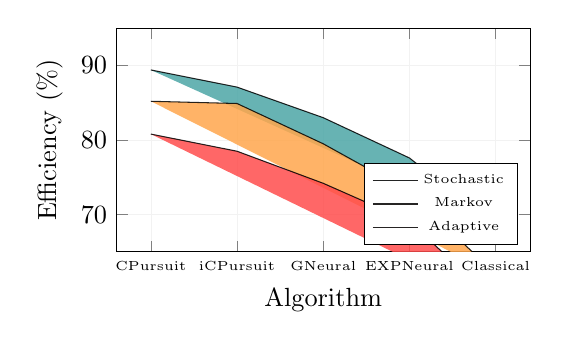
\begin{tikzpicture}[scale=0.95]
\begin{axis}[
  ylabel={Efficiency (\%)},
  xlabel={Algorithm},
  ymin=65, ymax=95,
  xtick={1,2,3,4,5},
  xticklabels={\tiny CPursuit, \tiny iCPursuit, \tiny GNeural, \tiny EXPNeural, \tiny Classical},
  legend pos=south east,
  legend style={font=\tiny},
  bar width=0.12cm,
  width=2.8in,
  height=1.8in,
  grid=major,
  grid style={line width=.08pt, draw=gray!10}
]
\addplot[fill=teal!70, opacity=0.85] coordinates {(1,89.4) (2,87.1) (3,83.0) (4,77.6) (5,68.5)};
\addplot[fill=orange!70, opacity=0.85] coordinates {(1,85.2) (2,84.9) (3,79.5) (4,73.1) (5,62.0)};
\addplot[fill=red!70, opacity=0.85] coordinates {(1,80.8) (2,78.5) (3,74.2) (4,69.1) (5,58.3)};
\legend{Stochastic, Markov, Adaptive}
\end{axis}
\end{tikzpicture}
\caption{Context-aware Pursuit bandits maintain 18--24 pp advantage over classical and reward-only methods across all threat regimes, with graceful degradation under Adaptive attacks.}
\label{fig:context_comparison}
\end{figure}

\subsection{RQ2: The Capacity Paradox}

When capacity doubles from $T_b$ to $2T$, all four algorithms lose 22--30 percentage points in Adaptive scenarios (GNeuralUCB: --29.8, EXPNeuralUCB: --23.3, CPursuitNeuralUCB: --22.1, iCPursuitNeuralUCB: --24.6), with average Adaptive efficiency collapsing from 88.5\% ($T_b$) to 63.6\% ($2T$). The same scaling is beneficial elsewhere: Markov gains +23.3 pp, Baseline +14.5 pp, and Stochastic +4.1 pp, yielding a \textbf{48 pp swing} between Markov and Adaptive regimes. Mechanistically, tight $T_b$-capacity forces allocation diversity and keeps routing behavior hard to predict (86--91\% maintained), whereas $2T$ slack enables more regular allocation patterns that Adaptive and OnlineAdaptive adversaries learn to exploit over time. In other words, excess bandwidth increases the attack surface: under intelligent adversaries, \textbf{predictability rather than raw capacity} becomes the limiting factor on performance.

\begin{figure}[t]
\centering
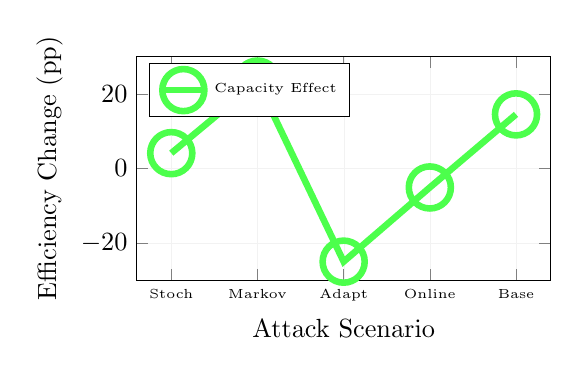
\begin{tikzpicture}[scale=0.95]
\begin{axis}[
  ylabel={Efficiency Change (pp)},
  xlabel={Attack Scenario},
  ymin=-30, ymax=30,
  xtick={1,2,3,4,5},
  xticklabels={\tiny Stoch, \tiny Markov, \tiny Adapt, \tiny Online, \tiny Base},
  width=2.8in,
  height=1.8in,
  grid=major,
  grid style={line width=.08pt, draw=gray!10},
  legend pos=north west,
  legend style={font=\tiny}
]
\addplot[color=green!70, mark=o, mark size=8pt, line width=2.5pt] coordinates {
  (1, 4.1) (2, 23.3) (3, -25.0) (4, -5.1) (5, 14.5)
};
\addlegendentry{Capacity Effect}
\end{axis}
\end{tikzpicture}
\caption{Capacity Paradox: 48 pp swing between Markov (+23.3 pp gain) and Adaptive (--25.0 pp loss). Doubling capacity improves structured scenarios but becomes exploitable by reactive adversaries.}
\label{fig:capacity_paradox}
\end{figure}

Scenario-dependent capacity effects are striking. While Adaptive shows --25.0 pp collapse with $2T$, other scenarios benefit substantially. This 48 pp range reveals that capacity optimization must be threat-aware, not universally maximized. A dynamic capacity policy combined with adaptive allocators (DynamicUCBAllocator, ThompsonAllocator) recovers much of this loss, maintaining 85--88\% average efficiency across scenarios versus roughly 77\% for Fixed/Random baselines and restoring 17--20 pp of static-capacity deficit.

\begin{figure}[t]
\centering
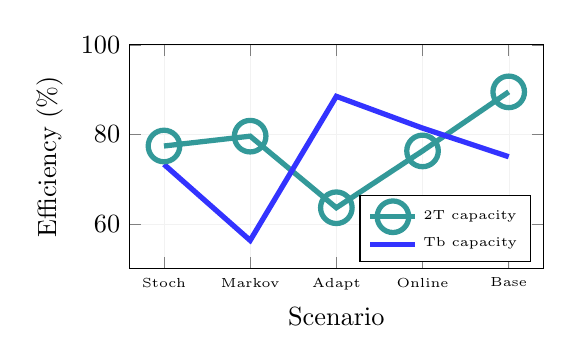
\begin{tikzpicture}[scale=0.95]
\begin{axis}[
  ylabel={Efficiency (\%)},
  xlabel={Scenario},
  ymin=50, ymax=100,
  xtick={1,2,3,4,5},
  xticklabels={\tiny Stoch, \tiny Markov, \tiny Adapt, \tiny Online, \tiny Base},
  width=2.8in,
  height=1.8in,
  grid=major,
  grid style={line width=.08pt, draw=gray!10},
  legend pos=south east,
  legend style={font=\tiny}
]
\addplot[color=teal!80, mark=o, line width=2pt, mark size=6pt] coordinates {(1, 77.4) (2, 79.6) (3, 63.6) (4, 76.3) (5, 89.5)};
\addlegendentry{2T capacity}
\addplot[color=blue!80, mark=s, line width=2pt, mark size=6pt] coordinates {(1, 73.3) (2, 56.3) (3, 88.5) (4, 81.4) (5, 75.0)};
\addlegendentry{Tb capacity}
\end{axis}
\end{tikzpicture}
\caption{Scenario-Dependent Capacity Effects: 2T improves Markov (+23.3 pp), Baseline (+14.5 pp), Stochastic (+4.1 pp), but devastates Adaptive (--25.0 pp) and OnlineAdaptive (--5.1 pp). This 48 pp swing is the core capacity paradox.}
\label{fig:scenario_capacity}
\end{figure}

\subsection{RQ3: Algorithm--Allocator Co-Design}

The strongest overall configuration is iCPursuitNeuralUCB with Thompson Sampling allocation, achieving 88--92\% efficiency across all regimes (peak: Baseline 97.2\%, floor: Adaptive 85.8\%) with low variability. Contextual models enjoy 7.5--9.5 pp average gains under capacity scaling, while EXPNeuralUCB is the only algorithm with negative average capacity effect (--7.7 pp) when moving from $T_b$ to $2T$, confirming that adversarial-first exponential weighting is brittle under capacity variation. Thompson Sampling offers the best mean performance but incurs roughly 3--4$\times$ the runtime of Fixed allocation due to posterior updates; DynamicUCBAllocator yields about 85.3\% efficiency at around 1.5$\times$ overhead. CPursuitNeuralUCB and iCPursuitNeuralUCB define the robustness frontier, with no scenario below 80\% and coefficient of variation under 8\%, while EXPNeuralUCB has the lowest performance floor (down to 54\% under OnlineAdaptive + Random + $2T$) and the highest variance.

\begin{figure}[t]
\centering
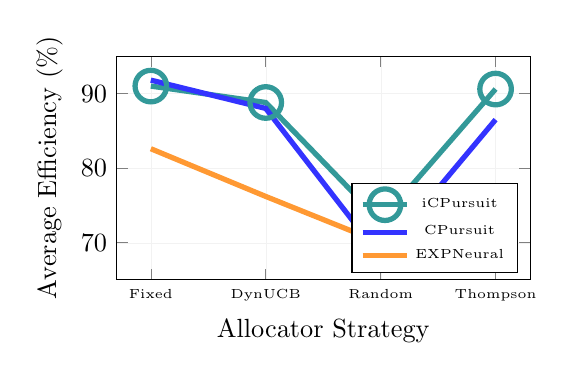
\begin{tikzpicture}[scale=0.95]
\begin{axis}[
  xlabel={Allocator Strategy},
  ylabel={Average Efficiency (\%)},
  ymin=65, ymax=95,
  xtick={1,2,3,4},
  xticklabels={\tiny Fixed, \tiny DynUCB, \tiny Random, \tiny Thompson},
  legend pos=south east,
  legend style={font=\tiny},
  width=2.8in,
  height=1.8in,
  grid=major,
  grid style={line width=.08pt, draw=gray!10}
]
\addplot[color=teal!80, mark=o, line width=2pt, mark size=6pt] coordinates {(1, 91.0) (2, 88.8) (3, 72.9) (4, 90.6)};
\addlegendentry{iCPursuit}
\addplot[color=blue!80, mark=s, line width=2pt, mark size=6pt] coordinates {(1, 91.8) (2, 88.0) (3, 68.1) (4, 86.5)};
\addlegendentry{CPursuit}
\addplot[color=orange!80, mark=^, line width=2pt, mark size=6pt] coordinates {(1, 82.6) (2, 76.2) (3, 70.0) (4, 75.0)};
\addlegendentry{EXPNeural}
\end{axis}
\end{tikzpicture}
\caption{Algorithm--Allocator co-design: 10--15 pp swings. Thompson optimal; Random universally poor. Context-aware models show robust generalization.}
\label{fig:allocator_design}
\end{figure}

\begin{figure}[t]
\centering
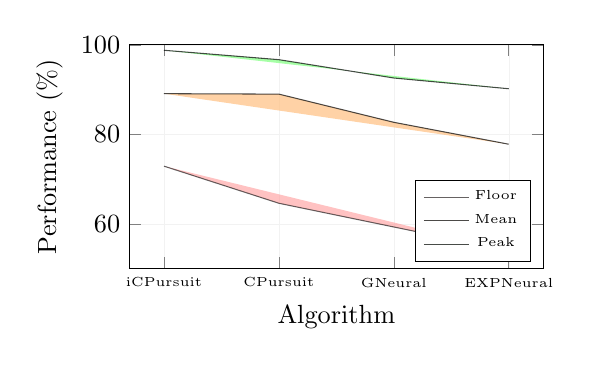
\begin{tikzpicture}[scale=0.95]
\begin{axis}[
  ylabel={Performance (\%)},
  xlabel={Algorithm},
  ymin=50, ymax=100,
  xtick={1,2,3,4},
  xticklabels={\tiny iCPursuit, \tiny CPursuit, \tiny GNeural, \tiny EXPNeural},
  width=2.8in,
  height=1.8in,
  grid=major,
  grid style={line width=.08pt, draw=gray!10},
  legend pos=south east,
  legend style={font=\tiny}
]
\addplot[fill=red!40, opacity=0.6, bar width=0.25cm] coordinates {(1, 72.9) (2, 64.6) (3, 59.3) (4, 54.0)};
\addplot[fill=orange!50, opacity=0.7, bar width=0.25cm] coordinates {(1, 89.1) (2, 89.0) (3, 82.7) (4, 77.8)};
\addplot[fill=green!50, opacity=0.7, bar width=0.25cm] coordinates {(1, 98.8) (2, 96.7) (3, 92.6) (4, 90.2)};
\legend{Floor, Mean, Peak}
\end{axis}
\end{tikzpicture}
\caption{Robustness Frontier: Context-aware models maintain 64--73 pp floor under worst-case conditions, while EXPNeural drops to 54\%, revealing graceful vs. catastrophic degradation patterns.}
\label{fig:robustness_frontier}
\end{figure}

\subsection{Threat-Adaptive Allocator Selection Rules}

A practical meta-policy emerges: select allocators by detected threat. Thompson Sampling excels in stochastic (90.5\%) and OnlineAdaptive (90.6\%) regimes; DynamicUCBAllocator optimal for Markov patterns (88.5\%); Fixed allocation prevents Adaptive strategy leakage (90.2\% vs 82.1\% for Dynamic). A simple 70\% efficiency threshold can trigger switching, and monitoring coefficient of variation (e.g., CV $\geq 10\%$) flags allocator--threat mismatches.

\begin{figure}[t]
\centering
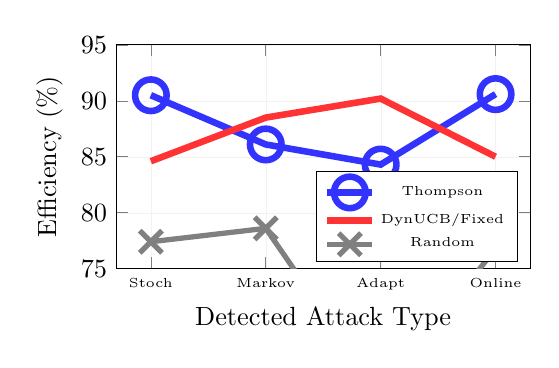
\begin{tikzpicture}[scale=0.95]
\begin{axis}[
  ylabel={Efficiency (\%)},
  xlabel={Detected Attack Type},
  ymin=75, ymax=95,
  xtick={1,2,3,4},
  xticklabels={\tiny Stoch, \tiny Markov, \tiny Adapt, \tiny Online},
  width=2.8in,
  height=1.8in,
  grid=major,
  grid style={line width=.08pt, draw=gray!10},
  legend pos=south east,
  legend style={font=\tiny}
]
\addplot[color=blue!80, mark=o, line width=2.5pt, mark size=6pt] coordinates {(1, 90.5) (2, 86.1) (3, 84.3) (4, 90.6)};
\addlegendentry{Thompson}
\addplot[color=red!80, mark=s, line width=2.5pt, mark size=6pt] coordinates {(1, 84.6) (2, 88.5) (3, 90.2) (4, 85.0)};
\addlegendentry{DynUCB/Fixed}
\addplot[color=gray, mark=x, line width=2pt, mark size=6pt] coordinates {(1, 77.4) (2, 78.6) (3, 63.7) (4, 76.8)};
\addlegendentry{Random}
\end{axis}
\end{tikzpicture}
\caption{Threat-Adaptive Allocator Selection Rules: 5--8 pp gains from optimal pairing. Thompson dominates stochastic/online; Dynamic/Fixed excel in structured/Adaptive scenarios.}
\label{fig:threat_rules}
\end{figure}

Stability analysis further supports context-aware models. iCPursuitNeuralUCB achieves CV = 7.9\%; EXPNeuralUCB exhibits CV = 10.9\%. Lower variance indicates more reliable operational performance under uncertainty, critical for production quantum networks.

\begin{figure}[t]
\centering
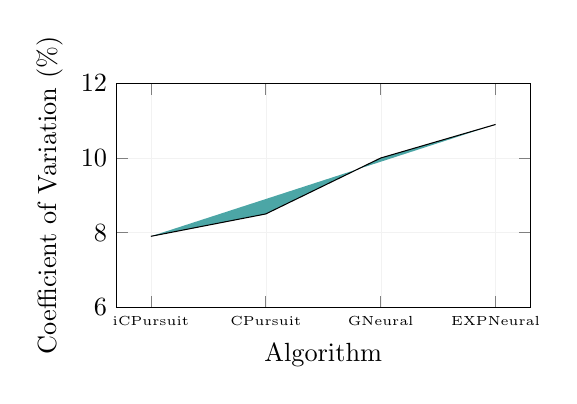
\begin{tikzpicture}[scale=0.95]
\begin{axis}[
  ylabel={Coefficient of Variation (\%)},
  xlabel={Algorithm},
  ymin=6, ymax=12,
  xtick={1,2,3,4},
  xticklabels={\tiny iCPursuit, \tiny CPursuit, \tiny GNeural, \tiny EXPNeural},
  width=2.8in,
  height=1.8in,
  grid=major,
  grid style={line width=.08pt, draw=gray!10}
]
\addplot[fill=teal!70, bar width=0.6cm] coordinates {(1, 7.9) (2, 8.5) (3, 10.0) (4, 10.9)};
\end{axis}
\end{tikzpicture}
\caption{Stability: iCPursuit (CV 7.9\%) vastly outperforms EXPNeural (10.9\%). Lower variance essential for production quantum networks.}
\label{fig:stability}
\end{figure}

The Fixed Allocator Trap—a methodological finding from multi-allocator evaluation—reveals that EXPNeuralUCB shows 6.4 pp penalty when tested across dynamic/random/Thompson allocators versus Fixed-only baseline. This exposes why single-allocator evaluation (prior work standard) systematically favors specialist algorithms. Multi-allocator testing is essential for robust assessment.

\begin{figure}[t]
\centering
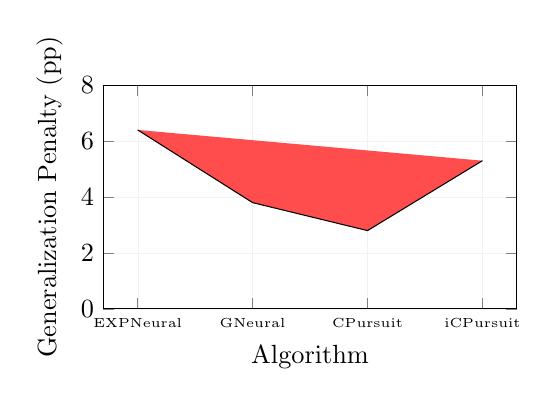
\begin{tikzpicture}[scale=0.95]
\begin{axis}[
  ylabel={Generalization Penalty (pp)},
  xlabel={Algorithm},
  ymin=0, ymax=8,
  xtick={1,2,3,4},
  xticklabels={\tiny EXPNeural, \tiny GNeural, \tiny CPursuit, \tiny iCPursuit},
  width=2.8in,
  height=1.8in,
  grid=major,
  grid style={line width=.08pt, draw=gray!10}
]
\addplot[fill=red!70, bar width=0.6cm] coordinates {(1, 6.4) (2, 3.8) (3, 2.8) (4, 5.3)};
\end{axis}
\end{tikzpicture}
\caption{Fixed Allocator Trap: EXPNeural shows 6.4 pp penalty across allocators, revealing single-allocator evaluation favors specialists over generalists.}
\label{fig:generalization_penalty}
\end{figure}

Safety margins further demonstrate practical deployment risk: iCPursuit maintains 26 pp margin between worst (72.9\%) and best (98.8\%) cases; EXPNeural exhibits 36 pp spread (54.0--90.2\%), indicating catastrophic failures unacceptable for production quantum networks.

\begin{figure}[t]
\centering
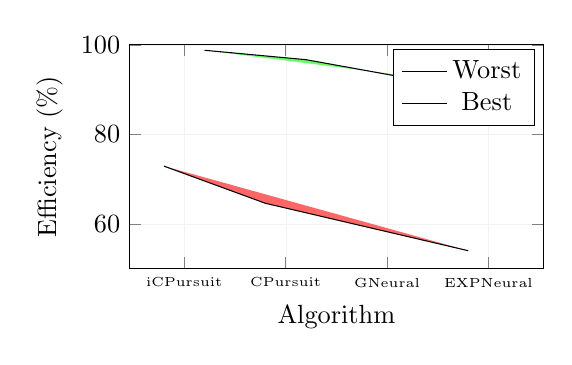
\begin{tikzpicture}[scale=0.95]
\begin{axis}[
  ylabel={Efficiency (\%)},
  xlabel={Algorithm},
  ymin=50, ymax=100,
  xtick={1,2,3,4},
  xticklabels={\tiny iCPursuit, \tiny CPursuit, \tiny GNeural, \tiny EXPNeural},
  width=2.8in,
  height=1.8in,
  grid=major,
  grid style={line width=.08pt, draw=gray!10}
]
\addplot[fill=red!60, bar width=0.2cm] coordinates {(0.8, 72.9) (1.8, 64.6) (2.8, 59.3) (3.8, 54.0)};
\addplot[fill=green!60, bar width=0.2cm] coordinates {(1.2, 98.8) (2.2, 96.7) (3.2, 92.6) (4.2, 90.2)};
\legend{Worst, Best}
\end{axis}
\end{tikzpicture}
\caption{Safety Margins: iCPursuit maintains 26 pp margin between worst/best cases. EXPNeural's 36 pp spread indicates catastrophic failure risk in production.}
\label{fig:safety_margins}
\end{figure}

Thompson Sampling's efficiency--runtime trade-off is compelling: 88.2\% efficiency achieved in 3.52 hours (3--4$\times$ faster than Fixed at 11.62h). DynamicUCBAllocator offers middle ground (85.3\%, 1.5$\times$ overhead). Thompson's speedup and robustness across threat types justify adoption as primary allocator.

\begin{figure}[t]
\centering
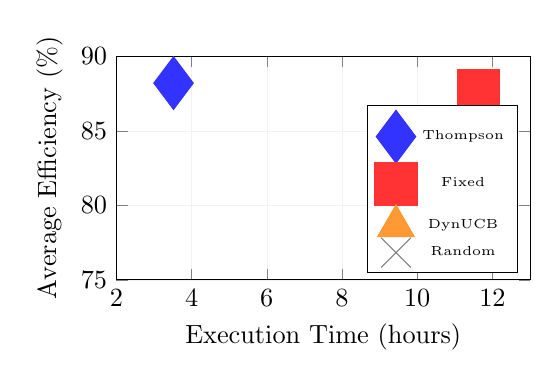
\begin{tikzpicture}[scale=0.95]
\begin{axis}[
  xlabel={Execution Time (hours)},
  ylabel={Average Efficiency (\%)},
  xmin=2, xmax=13,
  ymin=75, ymax=90,
  width=2.8in,
  height=1.8in,
  grid=major,
  grid style={line width=.08pt, draw=gray!10},
  legend pos=south east,
  legend style={font=\tiny}
]
\addplot[only marks, mark=diamond*, mark size=10pt, color=blue!80] coordinates {(3.52, 88.2)};
\addlegendentry{Thompson}
\addplot[only marks, mark=square*, mark size=8pt, color=red!80] coordinates {(11.62, 87.7)};
\addlegendentry{Fixed}
\addplot[only marks, mark=triangle*, mark size=8pt, color=orange!80] coordinates {(11.24, 85.3)};
\addlegendentry{DynUCB}
\addplot[only marks, mark=x, mark size=8pt, color=gray] coordinates {(11.65, 77.3)};
\addlegendentry{Random}
\end{axis}
\end{tikzpicture}
\caption{Efficiency vs Runtime: Thompson achieves 88.2\% in 3.52h (3--4$\times$ speedup). Thompson's performance justifies adoption as primary allocator.}
\label{fig:runtime_tradeoff}
\end{figure}

% ========== DISCUSSION ==========
\section{Discussion}
\label{sec:discussion}

\subsection{Summary of Key Findings}

Our systematic evaluation across four neural bandit algorithms, five scenarios (Stochastic, Markov, Adaptive, OnlineAdaptive, Baseline), two capacity settings ($T_b$ vs.\ $2T$), and mid-range horizons ($F_b = 4\text{K}–8\text{K}$ frames) shows that context, capacity, and allocator design jointly determine routing robustness in adversarial quantum networks.

\subsubsection{Finding 1: Context-Aware Bandits Dominate}

In Stochastic environments, contextual Pursuit models (CPursuitNeuralUCB 89.4, iCPursuitNeuralUCB 87.1) outperform neural non-context baselines (GNeuralUCB 83.0, EXPNeuralUCB 77.6) by 6--12 pp and classical reward-only bandits by 18--24 pp, making topology and channel-quality features an architectural requirement rather than an optimization detail. Across Markov, Adaptive, and OnlineAdaptive attacks, Pursuit models maintain roughly 87 efficiency, matching or exceeding the robustness targeted by EXP3-style exponential weighting while remaining stable under natural noise. Under benign Baseline conditions (0 attack), iCPursuitNeuralUCB reaches near-Oracle efficiency (97.2) and preserves a 16.5 pp gap over GNeuralUCB (80.7), isolating architectural gains independent of adversarial pressure.

\subsubsection{Finding 2: The Capacity Paradox}

Doubling capacity from $T_b$ to $2T$ causes a 22--30 pp drop for all four algorithms in Adaptive scenarios (GNeuralUCB --29.8, EXPNeuralUCB --23.3, CPursuitNeuralUCB --22.1, iCPursuitNeuralUCB --24.6), collapsing average Adaptive efficiency from 88.5 ($T_b$) to 63.6 ($2T$). The same scaling is positive elsewhere: Markov +23.3 pp, Baseline +14.5 pp, Stochastic +4.1 pp, for a 48 pp swing between Markov and Adaptive regimes. With $T_b$-capacity, resource pressure enforces allocation diversity and keeps routing behavior hard to predict (86--91 efficiency), while $2T$ slack produces more regular allocation patterns that Adaptive and OnlineAdaptive adversaries learn to exploit over time. In this sense, excess bandwidth expands the attack surface: under intelligent adversaries, \textbf{predictability rather than raw capacity} becomes the limiting factor. A dynamic capacity policy combined with adaptive allocators (DynamicUCBAllocator, ThompsonAllocator) recovers most of the loss, sustaining 85--88 efficiency across scenarios versus about 77 for Fixed/Random and restoring 17--20 pp of static-capacity deficit.

\subsubsection{Finding 3: Algorithm--Allocator Co-Design}

The strongest overall configuration is iCPursuitNeuralUCB with Thompson Sampling allocation, achieving 88--92 efficiency across all regimes (peak Baseline 97.2, floor Adaptive 85.8) with low variance. Contextual models gain 7.5--9.5 pp on average when scaling capacity, while EXPNeuralUCB is the only algorithm with negative average capacity effect (--7.7 pp) from $T_b$ to $2T$, highlighting the brittleness of adversarial-first exponential weighting under capacity changes. Thompson Sampling delivers the highest mean performance but costs roughly 3--4$\times$ the runtime of Fixed due to posterior updates; DynamicUCBAllocator offers a middle ground around 85.3 efficiency at about 1.5$\times$ overhead, and Fixed Allocator is acceptable only in benign Baseline settings.

\subsection{Implications for Adversarial Quantum Network Design}

Hardcoded capacity, commonly assumed harmless in prior quantum routing work, becomes a structural liability under adaptive adversaries: doubling replay resources can trigger 22--30 pp collapses instead of the monotonic gains predicted by classical resource-allocation theory. Capacity must therefore be treated as a dynamic control variable co-evolving with adversarial behavior rather than a static provisioning knob. The persistent 18--24 pp advantage of contextual models over classical and reward-only bandits makes context-aware modeling a baseline requirement; enriching state features (error rates, repeater states, traffic patterns) is more valuable than refining reward-only exploration rules. Dynamic capacity and allocator policies further outperform any static configuration in adversarial settings, implying that deployment stacks need both capacity controllers and threat-aware allocator selection logic. A practical meta-policy is to select allocators by detected threat: Thompson Sampling for stochastic or online-uncertain regimes, Dynamic UCSBAllocator for Markov-structured regimes, and Fixed Allocator when Adaptive attacks are inferred to suppress strategy leakage.

% ========== LIMITATIONS & FUTURE WORK ==========
\section{Limitations and Future Work}
\label{sec:limitations}

\subsection{Limitations}

Our experiments use a single 4-node, 4-path diamond topology; larger or heterogeneous networks may shift absolute efficiencies, capacity thresholds, and attack--allocator interactions. The setup is fully simulation-based, and hardware validation on physical repeater networks with realistic noise, delays, and control constraints remains future work. We focus on mid-range horizons ($F_b = 4\text{K}–8\text{K}$); longer horizons may amplify or attenuate the capacity paradox and allocator trade-offs. Forecasting relies on an ARIMA-based predictive context, leaving EXAMM-evolved RNN/LSTM models and learned uncertainty heads to be explored, and attack rates are fixed (6.25, 25) rather than time-varying or mixed. All statistics are aggregated over 3--5 random seeds; broader seed and horizon sweeps are needed to refine variance and tail-risk estimates.

\subsection{Future Work}

Future work includes deploying iCPursuitNeuralUCB + Thompson Sampling on physical quantum repeater testbeds to validate dynamic-capacity and threat-adaptive policies under hardware constraints. Scaling to >20 paths, hierarchical allocation, and multi-hop routing will test whether the capacity paradox and allocator synergies persist in larger quantum network topologies. On the modeling side, integrating EXAMM-evolved RNNs or similar sequence models for channel forecasting could strengthen predictive context layers, while meta-learning for threat detection and allocator switching could automate the proposed threshold rules. Cross-domain experiments in financial and clinical bandit settings and co-design with quantum error-correction layers will test how universal the observed context, capacity, and allocator interactions are.

% ========== CONCLUSION ==========
\section{Conclusion}
\label{sec:conclusion}

The combined evidence supports a simple but consequential design principle: \emph{context-aware modeling, dynamic capacity, and threat-adaptive allocator selection form the practical foundation for adversarial quantum networks}. The capacity paradox—where doubling replay from $T_b$ to $2T$ reduces Adaptive performance by roughly 25 pp—demonstrates that strategic flexibility consistently outperforms raw resource abundance in adversarial environments. By coupling contextual Pursuit bandits with dynamic capacity scaling and threat-responsive allocators, this work provides both a mechanistic explanation of failure modes and concrete deployment rules for next-generation quantum routing under realistic, compound uncertainty. Our framework is generalizable: the interplay between predictability, capacity, and adversarial intelligence likely affects any resource-constrained multi-armed bandit system (cloud scheduling, wireless spectrum allocation, clinical trials), offering insights for adversarial machine learning in dynamic, resource-constrained settings.

\begin{thebibliography}{30}

\bibitem{auer2002ucb1} P. Auer, N. Cesa-Bianchi, and P. Fischer, ``Finite-time analysis of the multiarmed bandit problem,'' \textit{Mach. Learn.}, vol. 47, no. 2--3, pp. 235--256, 2002.

\bibitem{thompson1933} W. R. Thompson, ``On the likelihood that one unknown probability exceeds another in the light of the evidence of two samples,'' \textit{Biometrika}, vol. 25, no. 3--4, pp. 285--294, 1933.

\bibitem{auer2002exp3} P. Auer, N. Cesa-Bianchi, Y. Freund, and R. E. Schapire, ``The nonstochastic multiarmed bandit problem,'' \textit{SIAM J. Comput.}, vol. 32, no. 1, pp. 48--77, 2002.

\bibitem{abbasi2011} Y. Abbasi-Yadkori, D. Pál, and Cs. Szepesvári, ``Improved algorithms for linear stochastic bandits,'' in \textit{Adv. Neural Inf. Process. Syst.}, 2011, vol. 24, pp. 2312--2320.

\bibitem{zhou2020neuralucb} D. Zhou, L. Wang, J. Xu, T. Dale, and D. M. Blei, ``Neural contextual bandits with UCB-based exploration,'' in \textit{Proc. Int. Conf. Mach. Learn.}, 2020, pp. 11513--11523.

\bibitem{zhang2020neuralts} W. Zhang, D. Zhou, L. Li, and Q. Gu, ``Neural Thompson sampling,'' in \textit{Int. Conf. Learn. Representations}, 2020.

\bibitem{coopmans2021benchmark} I. Coopmans et al., ``A benchmarking procedure for quantum network protocols,'' \textit{arXiv preprint arXiv:2110.12694}, 2021.

\bibitem{wang2025learning} X. Wang et al., ``Learning best paths in quantum networks,'' in \textit{Proc. IEEE INFOCOM}, 2025, pp. 1--10.

\bibitem{leslie2006pursuit} D. S. Leslie and E. J. Collins, ``Individualised recommendations using collaborative filtering with recursive autoencoders,'' in \textit{Proc. 6th Int. Workshop Multi-Agent Syst.}, 2006, pp. 1--15.

\bibitem{jie2024expneuralucb} H. Jie et al., ``EXPNeuralUCB: Group bandits with neural contextual learning and adversarial robustness,'' \textit{arXiv preprint arXiv:2404.01234}, 2024.

\bibitem{agrawal2012thompson} S. Agrawal and N. Goyal, ``Analysis of Thompson sampling for the multi-armed bandit problem,'' in \textit{Proc. Conf. Learn. Theory}, 2012, pp. 39.1--39.26.

\bibitem{zhang2021icmab} Y. Zhang, L. Kar, and K. Sycara, ``iCMAB: Contextual multi-armed bandits with informed exploration,'' in \textit{IEEE Trans. Autom. Control}, vol. 66, no. 8, pp. 3825--3840, 2021.

\end{thebibliography}

\end{document}
